%%\documentstyle[12pt,epsfig]{article}
%%\begin{document}

\section{Generic bioenergetics} 

generic\_bioenergetics is a frame work to 
\begin{enumerate}
  \item make multi stage modelling, based on independent sub stages
  \item model growth energy budgets for early life stages
\end{enumerate} 
generic\_bioenergetics delivers the particle\_state interface for IBMlib.
The main idea is to localize species specific properties in particular modules
to ensure portability to new species.
generic\_bioenergetics focuses on early life stages where the natural internal units 
are $\mu$g for weight, mm for length and seconds for time.
Currently, internal classes within generic\_bioenergetics have public scope (for the time being)

\subsection{Multi stage modelling} 

Multi stage modelling is handled by a light weight bundling module that 
combines independent stages described by classes in other modules. The multi stage module
offers a class has independent stage class instances as components. The multi stage module
manages which stage is currently active and handles overall attributes, like the survival chance
of the organism, place and time of origin. The multi stage module interacts with independent stages
via the particle\_sub\_state interface described below

\subsubsection{Componets} 

\begin{itemize}
  \item Decorators: implement interface particle\_sub\_state by loading specific 
  biological models/data from other contexts and compiling it into a
  behavioral model (like optimal feeding larvae, optimal\_forager.f).
  These module are generic, i.e. does not contain reference to a particular species.

  \begin{itemize}
  \item module feeding\_larval\_stage   
  \item module yolksac\_larval\_stage                    
  \item module released\_egg\_stage 
  \end{itemize}

  Decorators may also by themselves provide the full particle\_state interface in parallel
  with particle\_sub\_state interface. To use this, a module name conversion dummy should
  be used. Currently this is only available for the implementation optimal\_forager.f 
  implementating module feeding\_larval\_stage   


------------------------------
\item Specific biological models:

  These module contain data for a particular species, so that these modules 
  should be provided for each species. These modules are the only ones containing 
  parameters for a particular species, so that all species specific information
  is contained here.

  \begin{itemize}
  \item module egg\_properties                          
  \item module yolksac\_properties                   
  \item module larval\_properties    
  \end{itemize}
------------------------------
\item Auxillary modules/components:

  Provides generic auxillary functionality for generic\_bioenergetics
  \begin{itemize}
  \item particle\_state\_base 
  \item prey\_community
  \item numerical\_1d\_integrals
  \item feeding\_larval\_stage\_2\_particle\_state.f (name change wrapper module)
  \end{itemize}

\end{itemize}




% ----------------------------------------------------------------------------
\begin{figure}[p]   % [tbhp]
\begin{center}                                                 
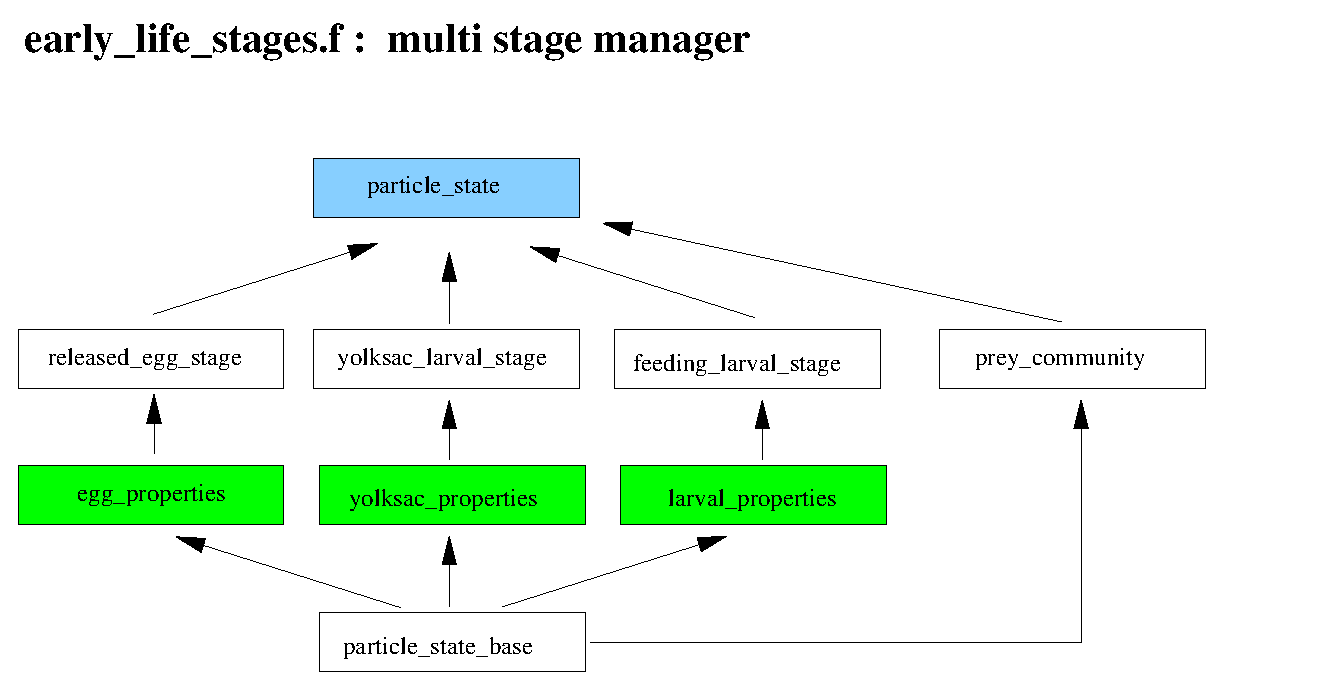
\epsfig{file=early_life_stages.eps,width=120mm,angle=0,clip=}     
\end{center}                                                    
\caption{Inheritance diagram for multi stage manager}
\label{multistagemanager:fig}
\end{figure}
% ----------------------------------------------------------------------------
% ----------------------------------------------------------------------------
\begin{figure}[p]   % [tbhp]
\begin{center}                                                  
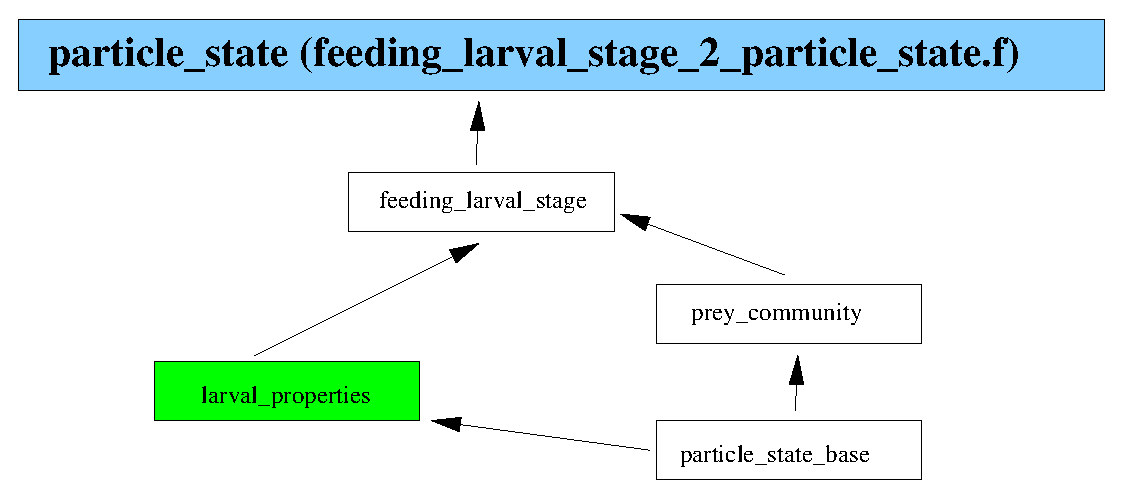
\epsfig{file=optimal_forager.eps,width=120mm,angle=0,clip=}        
\end{center}                                                    
\caption{Inheritance diagram for optimal foraging theory implementation of
         feeding\_larvae}
\label{feedinglarvae:fig}
\end{figure}
% ----------------------------------------------------------------------------


\subsubsection{particle\_sub\_state interface} 

The particle\_sub\_state interface is implemented by the decorator modules.
If X designates the stage (e.g. X=feeding\_larvae) then the particle\_sub\_state interface has the following 
components:
\begin{itemize}
  \item type X. This class is embedded in the multi stage class representing a multi staged organism.

 \item subroutine update\_particle\_state\_X(state, space, dt, mortality\_rate, die, next)  \newline
type(X), intent(inout)     :: state  \newline
type(spatial\_attributes), intent(inout) :: space  \newline
real,intent(in)                         :: dt ! in seconds  \newline
real,intent(out)                        :: mortality\_rate  \newline
logical,intent(out)                     :: die, next  \newline


 \item subroutine init\_state\_attributes\_X(state, space, time\_dir,  initdata)  \newline
type(X),intent(out)       :: state  \newline
type(spatial\_attributes),intent(inout) :: space  \newline
real,intent(in)                        :: time\_dir   \newline           
character*(*),intent(in)               :: initdata  \newline


 \item subroutine get\_active\_velocity\_X(state, space, v\_active)  \newline
type(X), intent(in)     :: state  \newline
type(spatial\_attributes), intent(in) :: space  \newline      
real, intent(out)                    :: v\_active(:) ! meter/second  \newline


\end{itemize}

Notes that the particle\_sub\_state interface is rather similar to the particle\_state interface, but that
update\_particle\_state\_X features extra output parameters mortality\_rate, die, next. These
parameters are needed by the multi stage manager to make stage transitions and manage overall
properties, like survival of the organism. The particle\_sub\_state interface for a particular stage will only
be applied if the stage is currently active.


\subsection{Growth energy budgets for early life stages} 

module feeding\_larval\_stage  in the implementation  optimal\_forager.f implements 
foraging based on optimal foraging theory (Charnov 1975). Diet switching is controlled completely by 
size-based processes in capture\_sucess, handling\_time, search\_volume provided by module larval\_properties. 
The continuous food spectrum is size based as provided by module prey\_community with prey\_spectrum\_density.
  
optimal\_forager.f can determine the maximal food intake (corresponding to the optimal diet) from a continuous food spectrum 
either by on-the-fly diet optimization or from a pretabulated data base of optimal diets for a reference database
set in the input file. The latter mode is for production runs, to avoid optimization for each organism in each 
time step. If the reference database is set appropriately, the results should be similar, to within numerical accuracy.
To set reference database, see input parameters for module feeding\_larval\_stage below.


\section{Module listing } 

%------------------------------------------------------------------------------------------------------------------
\subsection{Decorators} 
%------------------------------------------------------------------------------------------------------------------

\subsubsection{module feeding\_larval\_stage}                                     
implementation : optimal\_forager.f.
particle\_state interface/sub interface for feeding larval stage  
This version applies optimal foraging theory in relation to a size spectrum, based
on larval performance capture\_sucess/handling\_time/search\_volume
prescribed in module larval\_properties 

\begin{verbatim}
type feeding_larvae
      private
         type(larval_physiology) :: larvstate         ! defined in module larval_properties 
      end type
      public :: feeding_larvae ! make type state_attributes visible outside

 type state_attributes



      public :: init_particle_state  ! module operator
      public :: close_particle_state ! module operator
      public :: init_state_attributes
      public :: get_active_velocity
      public :: update_particle_state
      public :: delete_state_attributes 
      public :: write_state_attributes
      public :: get_particle_version
      public :: get_property         ! currently void
      public :: get_metadata_state   ! currently void

      public :: init_feeding_larval_stage
      public :: close_feeding_larval_stage
      public :: init_state_attributes_FL
      public :: get_active_velocity_FL
      public :: update_particle_state_FL
      public :: delete_state_attributes_FL
\end{verbatim}

Input parameters (for simulation file):\newline
\begin{itemize}
  \item ingestion\_integral\_sampling (integer). Diet integrals over
        size spectra are calculated using numerical integrals. This parameter
        tells how many sampling points are used for numerical integrals.  
  \item precalc\_ingestion\_DB (logical). Whether to generate a database of
        maximal intake (.true.) or calculate  maximal intake on the fly for each larvae in 
        each time step (.false.)
        If precalc\_ingestion\_DB is .true. then the following parameters
        specifying the reference database is generated
        \begin{itemize}
          \item larval\_length\_grid\_min (mm) feeding larval range, start
          \item larval\_length\_grid\_max (mm) feeding larval range, end
          \item larval\_length\_grid\_points (integer) sampling of larval range.
          \item logZ\_grid\_min (log(kg DW/m3)) Zooplankton range, start
          \item logZ\_grid\_max (log(kg DW/m3)) Zooplankton range, end
          \item logZ\_grid\_points (integer) sampling of zooplankton range.
          \item julian\_day\_grid\_points (integer) sampling of seasonal cycle
  \end{itemize}
\end{itemize}

%--------------------------------------------------------------------------------------
\subsubsection{module yolksac\_larval\_stage}                     implementation : yolksac\_larval\_stage.f

particle\_state sub interface for yolksac\_larval\_stage for
multi stage manager. Species specific properties comes from 
module yolksac\_properties     

\begin{verbatim}
type yolksac_larvae
      private
         real :: completion   ! 0 < completion < 1. Hatch at 1
      end type
      public :: yolksac_larvae ! make type state_attributes visible outside


c.....Particle sub state interface: (for multi stage manager)
      public :: init_yolksac_larval_stage  ! module operator
      public :: close_yolksac_larval_stage ! module operator
      public :: init_state_attributes_YL
      public :: get_active_velocity_YL
      public :: update_particle_state_YL
      public :: delete_state_attributes_YL
\end{verbatim}


%--------------------------------------------------------------------------------------
\subsubsection{module released\_egg\_stage}                        
implementation : released\_egg\_stage.f
particle\_state sub interface for released\_egg\_stage for
multi stage manager. Species specific properties comes from 
module yolksac\_properties     


\begin{verbatim}
type released_egg
      private
         real :: completion   ! 0 < completion < 1. Hatch at 1
      end type
      public :: released_egg ! make type state_attributes visible outside


c.....Particle sub state interface: (for multi stage manager)
      public :: init_released_egg_stage  ! module operator
      public :: close_released_egg_stage ! module operator
      public :: init_state_attributes_egg
      public :: get_active_velocity_egg
      public :: update_particle_state_egg
      public :: delete_state_attributes_egg

\end{verbatim}

%--------------------------------------------------------------------------------------
\subsubsection{module particle\_state}                             
implementation : early\_life\_stages.f
multi stage manager implementing particle\_state interface 
from merging sub interfaces

released\_egg\_stage + yolksac\_larval\_stage + feeding\_larval\_stage  


%======================================================================================
\subsection{Species specific modules}
%======================================================================================

These - currently three - modules are the only ones that contain species specific information.
When setting up a new species, it is these modules that should be implemented for a 
particular species. A good way to start is to look at an example implementation

%--------------------------------------------------------------------------------------
\subsubsection{module egg\_properties}                          
example implementation : sprat/sprat\_egg.f   
\begin{verbatim}
public ::  egg_devel_rate ! fraction/sec
\end{verbatim}

%--------------------------------------------------------------------------------------
\subsubsection{module yolksac\_properties}                     
example implementation : sprat/sprat\_yolksac\_larv.f
\begin{verbatim}
public ::  yolksac_absorb_rate  ! fraction/sec
\end{verbatim}
%--------------------------------------------------------------------------------------
\subsubsection{module larval\_properties}                       
example implementation : sprat/sprat\_feeding\_larv.f

TODO: deriva


\begin{verbatim}
type larval_physiology              ! component for state_attributes
         real    :: length          ! mandatory public entry: standard length in mm 
         real    :: weight          ! mandatory public entry: standard DW weight in myg 
end type

public :: init_larval_properties   ! module initialization
public :: close_larval_properties  ! module close down

public :: init_larval_physiology   ! class constructor
public :: close_larval_physiology  ! class destructor
public :: set_larvae_hatched       ! alternative class constructor

public :: length_to_nominal_weight ! length-weight key
public :: weight_to_nominal_length ! corresponding weight-length key
             
public :: capture_sucess           ! evaluate capture success of encounter 
public :: handling_time            ! evaluate handling time 
public :: search_volume            ! evaluate search volume            
public :: grow_larvae              ! update larval weight+length
public :: inquire_stage_change     ! inquire whether stage should change
public :: evaluate_mortality_rate  
\end{verbatim}

Dummy arguments in subroutine synopsis
\begin{itemize}
  \item lp: prey length (mm)
  \item llarv: larval length (mm)  
  \item local\_env: local environment object
  \item space: space attribute object for current position of the larvae
  \item weight:  larval weight ($\mu$g)
\end{itemize}    

Subroutine synopsis:
\begin{itemize}
  \item subroutine init\_larval\_properties() \newline
  \item subroutine close\_larval\_properties() \newline
  \item subroutine init\_larval\_physiology(self,llarv,weight) \newline
        set larval length llarv (mm) and weight ($\mu$g)
  \item subroutine close\_larval\_physiology(self) \newline
  \item subroutine set\_larvae\_hatched(self, space)  \newline
  \item subroutine length\_to\_nominal\_weight(llarv, weight) \newline
  \item subroutine weight\_to\_nominal\_length(weight, llarvh) \newline

  \item subroutine capture\_sucess(lp, llarv, local\_env, csuc, dcsuc\_dlp) \newline
        prey capture success csuc (propability) and optionally its derivative wrt. lp: dcsuc\_dlp

  \item subroutine handling\_time(lp, llarv, local\_env, ht, dht\_dlp) \newline
        prey handling time ht [seconds] and optionally its derivative wrt. lp: dht\_dlp
  \item subroutine search\_volume(lp, llarv, local\_env, svol, dsvol\_dlp) \newline
        Search volume svol (unit = mm3/sec) of larvae with length llarv
        wrt. prey of length lp and optionally its derivative wrt. lp: dsvol\_dlp)
  \item subroutine grow\_larvae(self, local\_env, irate, dt) \newline 
        Update larval mass and length corresponding to interval dt
        subject to (maximal) ingestion rate.    
  \item subroutine inquire\_stage\_change(self, next) \newline
        Test whether to advance (or regress) ontogenetic stage 
        Return next = .true. to advance (or regress) to ontogenetic stage (depending on sign of dt)
        Do not consider sign of simulation time arrow
        assumes weight/length are appropriately updated
  \item subroutine evaluate\_mortality\_rate(self, local\_env, mortality\_rate, die) \newline
        Based on the current state and in the current environment
        evaluate the current mortality\_rate and wheter the larvae 
        should die (logical) absolutely (avoid setting mortality\_rate = infinity) 
\end{itemize}     



%======================================================================================
\subsection{Auxillary modules}
%======================================================================================

\subsubsection{module particle\_state\_base}                                      
implementation : particle\_state\_base.f
generic services for particle\_state implementations

\begin{verbatim}
type local_environment   ! cache local environment to avoid multiple identical interpolations of physical environment

public :: probe_local_environment
public :: write_local_environment
public :: clear_local_environment
\end{verbatim}

%------------------------------------------------------------------------------------------------------------------
\subsubsection{module prey\_community}                                           
implementation : prey\_community.f

reconstruct prey size spectrum
\begin{verbatim}
public :: prey_mass                ! length-weight key for prey
public :: prey_spectrum_density    ! evaluate size spectrum 
\end{verbatim}
%------------------------------------------------------------------------------------------------------------------
\subsubsection{module particle\_state}                                           
implementation: feeding\_larval\_stage\_2\_particle\_state.f
transparent wrapper to change name of module feeding\_larval\_stage to particle\_state      



%% \end{document}
